% !TEX encoding = UTF-8
% !TEX TS-program = pdflatex
% !TEX root = computabilità e algoritmi.tex
% !TEX spellcheck = it-IT
\section{Ordinamento topologico}\label{ordinamento-topologico}

Un \textbf{ordinamento topologico} definito su un grafo orientato
aciclico (\textbf{DAG}) è un ordinamento dei suoi vertici tale che per
ogni arco $uv \in E$, il vertice \emph{u} precede il vertice
\emph{v}.

\begin{figure}[htbp]
\centering
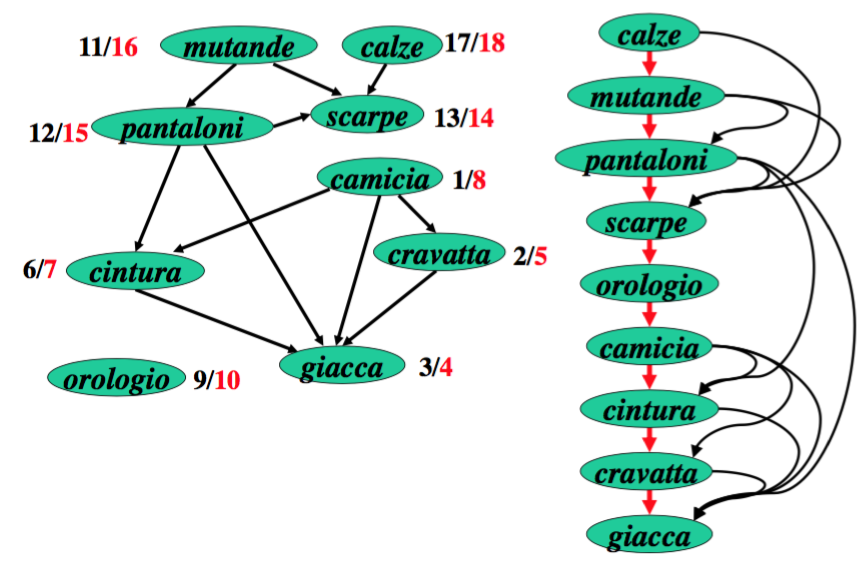
\includegraphics[width=0.6\textwidth]{./notes/immagini/l7-fig1.png}
\caption{Esempio di DAG}
\end{figure}

L'algoritmo effettua una ricerca in profondità e una volta completata la
visita di un nodo, lo inserisce in cima alla pila, ottenendo così una
pila ordinata per tempo di finitura decrescente.

\begin{breakablealgorithm}
	\caption{TS: ordinamento topologico di un grafo}
	\begin{algorithmic}[1]
		\Function{TS}{$ G $}
			\For{$ \forall v \in G.V $}
				\State $ v.color \gets bianco $
			\EndFor
			\State $ P \gets \emptyset $
			\For{$ \forall v \in G.V $}
				\If{$ v.color = bianco $}
					\State \textsc{TS-Visit}$ (G,v,P) $
				\EndIf
			\EndFor
			\State \Return $ P $
		\EndFunction
		\Statex
		\Function{TS-Visit}{$ G,u,P $}
			\State $ u.color \gets grigio $
			\For{$ \forall v \in Adj[u] $}
				\If{$ v.color = bianco $}
					\State \textsc{TS-Visit}$ (G,v,P) $
				\EndIf
			\EndFor
			\State $ u.color \gets nero $
			\State \textsc{PUSH}$ (P,u) $
		\EndFunction
	\end{algorithmic}
\end{breakablealgorithm}

La complessità dell'algoritmo è la stessa della visita in profondità,
ovvero \emph{O(n+m)}.

\subsection{Correttezza di TS}\label{correttezza-di-ts}

Per dimostrare la correttezza di \textsc{TS} è necessario dimostrare che
per ogni arco \emph{uv} il vertice \emph{v} viene finito prima del
vertice \emph{u}, ovvero \emph{u} si trova più in alto nella pila
rispetto a \emph{v}.

Prima di tutto è necessario dimostrare che un grafo è un \textbf{DAG} se
e solo se nella visita in profondità non si trova nessun arco
all'indietro e questo può essere fatto in modo analogo a come avviene
per un grafo non orientato.

Ovvero, se in una visita in profondità si trova un arco all'indietro \textit{vu}, 
allora tale arco aggiunto al cammino da \textit{u} a \textit{v} forma un ciclo.
Il cammino tra \textit{u} e \textit{v} esiste perché \textit{v} è discendete di \textit{u}.

Viceversa, supponendo che il grafo abbia un ciclo. 
Sia \textit{v} il primo vertice del ciclo ad essere scoperto e
sia \textit{uv} l’arco del ciclo che entra in \textit{v}.
Quando \textit{v} viene scoperto esiste un cammino bianco da \textit{v} ad \textit{u} e quindi, per la proprietà del cammino bianco, \textit{u} è discendente di \textit{v}.
Di conseguenza \textit{uv} è un arco all’indietro.

Tornando alla correttezza di \textsc{TS}, quando viene esplorato l'arco
\emph{uv}, il vertice \emph{u} è grigio e il vertice \emph{v} non può
essere grigio, altrimenti \emph{uv} sarebbe un arco all'indietro.

Se \emph{v} è nero, vuol dire che è già stato finito, mentre \emph{u}
non lo è, quindi \emph{u} viene inserito più in alto nella pila rispetto
a \emph{v}.

Se \emph{v} è bianco, per il teorema del cammino bianco, è anche un
discendente di \emph{u} e quindi viene finito prima di \emph{u} e di
conseguenza \emph{v} si trova più in basso nella pila rispetto a
\emph{u}.

\section{Componenti fortemente connesse}\label{componenti-fortemente-connesse}

La visita in profondità può essere utilizzata per individuare le
componenti fortemente connesse, ovvero i gruppi di nodi del grafico che
sono mutualmente raggiungibili tra di loro.

L'algoritmo che calcola le componenti fortemente connesse lavora in 3
passi:

\begin{enumerate}
\item
  Visita in profondità del grafo \emph{G} per ordinare i vertici in
  ordine di finitura decrescente, un po' come avviene nell'ordinamento
  topologico, con la differenza che non è garantita l'assenza di cicli.
\item
  Calcola il grafo trasposto $G^T$.
\item
  Visita in profondità il grafo trasposto $G^T$ usando l'ordine
  dei vertici nell'ordine calcolato al punto 1.
\end{enumerate}

Gli alberi della foresta così calcolata rappresentano le componenti
fortemente connesse.

La complessità dell'algoritmo è sempre \emph{O(n+m)}, perché tutti e 3 i
passi hanno complessità \emph{O(n+m)}.

\begin{figure}[htbp]
\centering
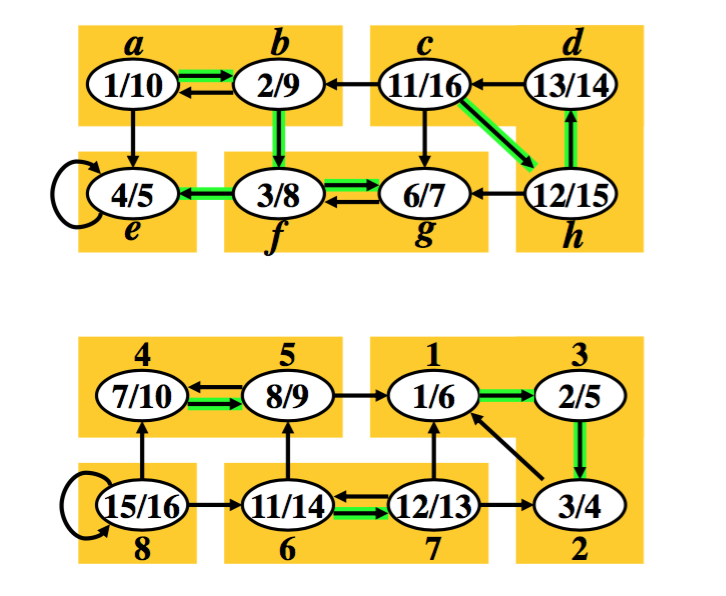
\includegraphics[width=0.6\textwidth]{./notes/immagini/l7-fig2.png}
\caption{Ricerca in profondità sul grafo di partenza e su quello di
trasposto. In verde la relazione padre-figlio. I numeri dei nodi nel
grafo trasposto indicano l'ordine di visita.}
\end{figure}

La dimostrazione di correttezza dell'algoritmo viene dopo perché si basa
su determinate proprietà che devono essere dimostrate.

\subsection{Proprietà dei cammini}\label{proprietuxe0-dei-cammini}

Siano \emph{C} e \emph{C'} due \textbf{CFC} distinte. Se esiste un
cammino $P_{uu'}$ da un vertice \emph{u} di \emph{C} ad un vertice
di \emph{u'} di \emph{C'}, non esiste nessun cammino $P_{vv'}$ da un
vertice di \emph{v'} di \emph{C'} a un vertice \emph{v} di \emph{C}.

La dimostrazione è banale, perché se ci fosse il cammino $P_{vv'}$
ci sarebbe un ciclo tra le due \textbf{CFC} e quindi queste non
sarebbero distinte, il che contraddice l'ipotesi.

\subsection{Proprietà dei tempi di fine}\label{prorpietuxe0-dei-tempi-di-fine}

Dato un insieme di vertici $ U \subseteq V $, \textit{d(U)} indica il tempo in cui viene scoperto il primo vertice in \textit{U}, mentre \textit{f(U)} indica il tempo in cui viene terminata l'esplorazione dell'ultimo vertice in \textit{U} durante la visita in profondità.

Si ha quindi che:

$$
d(U) = \min_{u \in U} (u.d) \: \text{e} \: f(U) = \max_{u \in U}(u.f)
$$

Siano \emph{C} e \emph{C'} due \textbf{CFC} distinte. Se esiste un arco
\emph{uv} da $u \in C$ a $v \in C'$, allora $f(C) > f(C')$, ovvero tutti i vertici di \emph{C}
vengono finiti prima dei vertici di \emph{C'}.

Possono quindi verificarsi due casi, ovvero che viene prima scoperto un
vertice di \emph{C} o di \emph{C'}.

Se $d(C) < d(C')$, quando viene scoperto il primo vertice
\emph{x} tutti i vertici, sia di \emph{C} che di \emph{C'} sono bianchi.
Quindi c'è un cammino bianco da \emph{x} a tutti i vertici di \emph{C}
e, a causa dell'arco \emph{uv}, c'è anche un cammino bianco da \emph{x}
a tutti i vertici di \emph{C'}. Per il teorema del cammino bianco, tutti
i vertici di \emph{C} e \emph{C'} diventeranno discendenti di \emph{x} e
quindi $x.f = f(C) > f(C')$.

Se $ d(C) > d(C') $, quando viene scoperto il primo vertice \textit{y} di \textit{C'}, tutti i vertici di \textit{C} e di \textit{C'} sono bianchi.
C'è quindi un cammino bianco da \textit{y} ad ogni vertice di \textit{C'} e quindi $ y.f = f(C') $.
Siccome esiste l'arco \textit{uv} non può esister nessun cammino da un vertice di \textit{C'} ad un vertice di \textit{C}, quindi \textit{C} non è raggiungibile da \textit{y}, dunque $ d(C) > f(C') $ e a maggior ragione $ f(C) > f(C') $

Come conseguenza di ciò si ha che se \textit{C} e \textit{C'} sono due \textbf{CFC} distinte del grafo \textit{G} e se nel grafo trasposto $ G^T $ esiste un arco \textit{uv} da $ u \in C$ a $ v \in C' $, allora $ f(C) < f(C') $ nella visita in profondità del grafo originale.
Questo perché le \textbf{CFC} del grafo originale sono le stesse del grafo trasposto e la presenza di $ uv \in G^T.E $ implica che $ vu \in G.E$, quindi per quanto precedentemente dimostrato $ f(C) < f(C') $ (considerando il grafo \textit{G}).

\subsection{Correttezza dell'algoritmo}\label{correttezza-dellalgoritmo}

La visita in profondità di $G^T$ parte dal vertice $x_1$
terminato per ultimo dalla visita in profondità di \emph{G}. Questo
vertice farà parte di una certa componente connessa $C_1$.

Si ha quindi che $x_1.f = f(C_1) > f(C)$ (nel grafo di partenza), pertanto non esiste $uv \in G.E$ da $ u \in C $ a $ v \in C' $ (proprietà dei tempi di fine) e quindi non esiste
nessun arco \emph{vu} in $G^T.E$ da $v \in C_1$ a $u \in C$ e di conseguenza l'albero costruito a partire da $x_1$ conterrà tutti e
soli i verti di $C_1$.

Dopodiché l'algoritmo continua da $x_2$ tra quelli terminati per
ultimi e che non sono $C_1$, sul quale è possibile fare lo
stesso ragionamento.

Questo continua fino a che non vengono visitati tutti i nodi, ottenendo
così una foresta di alberi che sono componenti fortemente connesse.

\subsection{(Esercizio) Componenti fortemente connesse e modifiche agli archi}\label{esericizio-componenti-fortemente-connesse-e-modifiche-agli-archi}

Come variano le componenti fortemente connesse aggiungendo un arco?
Trovare un esempio in cui il numero di \textbf{CFC} non cambia e un
esempio in cui il numero di \textbf{CFC} diminuisce di 1 ed un esempio
in cui il numero di \textbf{CFC} da 10 diventa 1.

\begin{itemize}
	\item \textbf{Non cambia} se aggiungo un arco che collega due nodi della stessa componente connessa oppure se aggiungo un arco \textit{uv} tra due vertici appartenenti a \textbf{CFC} distinte, $ v \in C $ e $ u \in C' $, tali che \textbf{non esiste} un cammino che collega un vertice di \textit{C'} a  uno di\textit{C}.
	\item \textbf{Diminuisce di 1} se aggiungo un arco \textit{uv} tra due vertici appartenenti a \textbf{CFC} distinte, $ v \in C $ e $ u \in C' $, tali che \textbf{esiste} un cammino che collega un vertice di \textit{C'} a uno di \textit{C}.
	\item \textbf{Da 10 diventa 1} se ad un cammino di 10 vertici aggiungo un arco che collega l'ultimo vertice del cammino con il primo.
\end{itemize}

\subsection{Grafo delle componenti fortemente connesse}\label{grafo-delle-componenti-fortemente-connesse}

Sia \emph{G} un grafo orientato per il quale sono state calcolate le
componenti fortemente connesse, indicate con $C_i$.

Si può definire il grafo delle componenti fortemente connesse, il quale ha come vertici i vari $C_i$ e come archi:

$$ 
E = \{xy | \exists uv \in G.E, \: x,u \in C_i, \: y,v \in C_j\}
$$

Il grafo così ottenuto astrae i cicli del grafo di partenza e risulta essere un \textbf{DAG}.

\subsubsection{Esercizio - Grafi semi-connessi}\label{esercizio---grafi-semiconnessi}

Un grafo orientato è semi-connesso se per ogni due vertici \emph{u} e
\emph{v} esiste o un cammino da \emph{u} a \emph{v} oppure un cammino da
\emph{v} a \emph{u}. Trovare un algoritmo efficiente per verificare se
un grafo è semi-connesso.

Questo può essere fatto costruendo il grafo delle componenti fortemente
connesse.

Se questo grafo contiene un cammino che connette tutti i suoi vertici allora il grafo è semplicemente connesso.

Per trovare il cammino basta ordinare topologicamente il grafo e verificare se da ogni componente c'è un arco che la connette alla componente successiva secondo l'ordine topologico.

Questo perché quando c'è un cammino tra tutte le CFC, si ha esiste un cammino tra tutti i nodi di una CFC a tutti i nodi di tutte le altre CFC.

Bisogna ora dimostrare che se non c'è questo cammino il grafo non è semi-connesso, supponendo che non ci sia un arco tra la componente \textit{i} e la componente \textit{i+1}.

Per come viene definito l'ordine topologico, se non c'è l'arco $i \rightarrow i+1$, vuol dire che non ci sono altri archi entranti nel vertice \textit{i+1}, pertanto non è possibile trovare alcun cammino che dal vertice \textit{i} in grado di raggiungere il vertice \textit{i+1}, passando anche per altri vertici del grafo.